\appendix
\counterwithin{equation}{section}
\renewcommand{\theequation}{\thesection.\arabic{equation}}

\section{证明}
\label{app:proofs}

\subsection{后代与报告模型}
\label{app:model}

成功次数为 $r$、成功概率为 $p$ 的负二项分布 $\NB(r,p)$ 的均值为 $r(1-p)/p$，方差为 $r(1-p)/p^2$。令 $r=k$、$p=k/(k+R_t)$，即得式~(\ref{eq:offspring})。$n$ 个相互独立的 $\NB(k,p)$ 变量之和服从 $\NB(nk,p)$；以保留概率 $\rho$ 对 $\NB(r,k/(k+\mu))$ 作二项稀疏化，得到 $\NB(r,k/(k+\rho\mu))$。结合这两条性质即得式~(\ref{eq:observed})。

\subsection{当期目标量}
\label{app:target1}

记 $C_t$ 的观测值为 $c$。由式~(\ref{eq:observed})，给定 $n$ 时 $R_t$ 的对数似然为
\begin{equation}
  \ell(R_t)=\text{const}+nk\log\frac{k}{k+\rho R_t}+c\log\frac{\rho R_t}{k+\rho R_t},
\end{equation}
相应的得分函数可写为
\begin{equation}
  \dot{\ell}(R_t)=\frac{c}{R_t}-\frac{(c+nk)\rho}{k+\rho R_t}=\mathcal{I}(R_t)\,(\Rhat_t-R_t),\qquad
  \mathcal{I}(R_t)=\frac{n}{R_t/\rho+R_t{}^2/k},
  \label{eq:score}
\end{equation}
其中 $\mathcal{I}(R_t)$ 为 Fisher 信息。$\Rhat_t=c/(\rho n)$ 的条件均值为 $R_t$，条件方差为 $R_t/(\rho n)+R_t{}^2/(kn)=1/\mathcal{I}(R_t)$。由于得分函数与 $\Rhat_t-R_t$ 成正比，对任意有限的 $n$，Cram\'er--Rao 下界均可达到。式~(\ref{eq:observed}) 中的分布是关于 $C_t$ 的单参数指数族，其自然参数 $\log[\rho R_t/(k+\rho R_t)]$ 的取值范围为一个开区间，因此 $C_t$ 为完备充分统计量，由 Lehmann--Scheff\'e 定理，$\Rhat_t$ 为 $R_t$ 的一致最小方差无偏估计量\citep{lehmann1998theory, lehmann2005testing}。

\subsection{命题~\ref{prop:average} 的证明}
\label{app:prop1}

记 $U=\Rbar^2+v_R$。在假设 H4 下，$\E(R_t\mid n)=\Rbar$，$\Var(R_t\mid n)=v_R$。由全方差公式与附录~\ref{app:target1} 的结果，误差方差为
\begin{equation}
  V(n,\rho)=\E\!\left[\frac{R_t}{\rho n}+\frac{R_t{}^2}{kn}\right]+\Var(R_t)=v_R+\frac{\Rbar}{\rho n}+\frac{U}{kn},
\end{equation}
代入 $m=\rho n$ 即得式~(\ref{eq:var-average})，其中 $A=A(\rho)=\Rbar+\rho U/k$ 依赖于 $\rho$。结论（i）与（ii）由取极限得到；固定 $n$ 时 $\rho$ 至多取 1，可达下限为 $v_R+\Rbar/n+U/(kn)$。

对于结论（iii），固定 $\rho$、$k$ 与 $R_t$ 的分布，经由 $n$ 改变 $m$，则 $A$ 为常数，$V(m;\rho)=v_R+A/m$，于是
\begin{equation}
  \frac{V(m;\rho)-V(2m;\rho)}{V(m;\rho)}=\frac{A/(2m)}{v_R+A/m}=\frac{1}{2(1+m/\mx)},
\end{equation}
在 $m=\mx$ 处等于四分之一。若改为固定 $n$ 而把 $\rho$ 增至 $2\rho$（$\rho\le1/2$），只有报告项 $\Rbar/(\rho n)$ 减半，方差的绝对降幅为 $\Rbar/(2\rho n)$，相对降幅为 $\Rbar/[2\rho nV(n,\rho)]$；后代项 $U/(kn)$ 不变，因此上式不适用于这一路径。$\rho$ 随路径变化时 $A$ 也随之变化，不能作为跨 $\rho$ 的常数。两条路径的对数边际为
\begin{equation}
  -\frac{\partial V}{\partial\log n}=\frac{\Rbar}{\rho n}+\frac{U}{kn}=\frac{A}{m},\qquad
  -\frac{\partial V}{\partial\log\rho}=\frac{\Rbar}{\rho n}=\frac{\Rbar}{m},
\end{equation}
二者之比为 $A/\Rbar$。

对于结论（iv），设 $\tilde{\theta}$ 为基于第 $t$ 期数据且满足 $\E(\tilde{\theta}\mid R_t)=R_t$ 的任一估计量，则 $\E(\tilde{\theta}-\Rbar)^2=\E[\Var(\tilde{\theta}\mid R_t)]+v_R\ge\E[1/\mathcal{I}(R_t)]+v_R=V$，取 $\Rhat_t$ 时等号成立。当 $R_{t+1}$ 与历史独立时，对 $y=C_{t+1}/m$ 作一步预测，有 $\E(\hat{y}-y)^2=(\hat{y}-\E y)^2+\Var(y)\ge V$，且在 $\hat{y}=\Rbar$ 处取等号。若 $R_t$ 为平稳一阶自回归过程，其方差为 $v_R$，相邻时期的相关系数为 $\phi$，则给定 $R_t$ 时 $R_{t+1}$ 的最优线性预测的误差方差为 $(1-\phi^2)v_R$\citep{hamilton1994time}。对于方差同为 $v_R$、平均两两相关系数为 $\bar{c}$ 的 $J$ 个辖区，其均值的方差为 $J^{-2}[Jv_R+J(J-1)\bar{c}v_R]$，由此得到式~(\ref{eq:pooling})。

\subsection{命题~\ref{prop:report-noise} 的证明}
\label{app:prop2}

记 $\sigma^2=\Var(p_t)=\tau^2\rho^2$。给定 $(n,R_t,p_t)$ 时，$C_t$ 的均值为 $p_tnR_t$，方差为 $p_tnR_t+p_t{}^2nR_t{}^2/k$。对 $p_t$ 取平均，给定 $(n,R_t)$ 的条件方差为
\begin{equation}
  \Var(C_t\mid n,R_t)=\rho nR_t+\frac{(\rho^2+\sigma^2)nR_t{}^2}{k}+\sigma^2n^2R_t{}^2.
\end{equation}
条件均值为 $\rho nR_t$，因此 $\Rhat_t$ 仍是 $\Rbar$ 的无偏估计量。再对 $R_t$ 取平均并除以 $(\rho n)^2$，得
\begin{equation}
  V_H(m)=v_R+\tau^2(\Rbar^2+v_R)+\frac{\Rbar}{m}+\frac{\rho(1+\tau^2)(\Rbar^2+v_R)}{km},
\end{equation}
此即式~(\ref{eq:vH-AH})。记 $U_H=(1+\tau^2)(\Rbar{}^2+v_R)$，则极限误差方差为 $v_R+v_H=U_H-\Rbar{}^2$，且 $A_H=\Rbar+\rho U_H/k$，因此 $\Rhat_t$ 的均值与方差仅通过 $U_H$ 依赖于 $v_R$ 与 $\tau$。不等式 $m_{\times,H}<\mx$ 等价于 $\rho v_R/k<A$；由于 $\Rbar^2+v_R>v_R$，后一不等式成立。

\subsection{命题~\ref{prop:allocation} 的证明与报告概率路径}
\label{app:prop3}

给定 $(R_1,\dots,R_T)$ 时，不同时期的病例数相互独立。记 $\bar{R}_T=T^{-1}\sum_tR_t$，则均值估计的方差为
\begin{equation}
  \Var\!\Big(\frac{1}{T}\sum_{t=1}^T\Rhat_t\Big)=\Var(\bar{R}_T)+\frac{A}{Tm},
\end{equation}
其中各期独立时 $\Var(\bar{R}_T)=v_R/T$，由此得到式~(\ref{eq:alloc-indep})。对于满足 $\Cov(R_s,R_t)=v_R\phi^{|s-t|}$ 的平稳一阶自回归过程，有 $T^2\Var(\bar{R}_T)=v_R[T+2\sum_{h=1}^{T-1}(T-h)\phi^h]$，对几何级数求和即得式~(\ref{eq:ar-sum})\citep{hamilton1994time}。固定 $\rho$，将 $T=\mathcal{B}/(c_0+c_1m)$ 代入式~(\ref{eq:alloc-indep})，得到目标函数
\begin{equation}
  f(m)=\frac{(c_0+c_1m)(v_R+A/m)}{\mathcal{B}},\qquad
  f'(m)=\frac{c_1v_R-c_0A/m^2}{\mathcal{B}},\qquad
  f''(m)=\frac{2c_0A}{\mathcal{B}m^3}>0.
\end{equation}
当 $c_0,c_1,v_R,A>0$ 时 $f$ 在 $m>0$ 上严格凸，唯一驻点满足 $m^{*2}=c_0A/(c_1v_R)=(c_0/c_1)\mx$，即式~(\ref{eq:optimal-m})。整数时期数、最低时期数与规模上限另作约束时，须把内点解与边界解比较；$v_R=0$ 时不存在有限内点解。

固定 $n$ 而改变 $\rho$ 时，令 $H=v_R+U/(kn)$、$Q=\Rbar/n$，单期方差为 $H+Q/\rho$。对单期成本 $c(\rho)>0$，目标函数与导数为
\begin{equation}
  f(\rho)=\frac{c(\rho)(H+Q/\rho)}{\mathcal{B}},\qquad
  f'(\rho)=\frac{c'(\rho)(H+Q/\rho)-c(\rho)Q/\rho^2}{\mathcal{B}}.
\end{equation}
成本函数未给定时不存在通用的最优报告概率。若 $c(\rho)=c_0+c_\rho\rho$，由 $f'(\rho)=0$ 得 $c_\rho H\rho^2=c_0Q$，即内点解 $\rho^*=\sqrt{c_0Q/(c_\rho H)}$，再截取到 $(0,1]$。若成本仍按 $c_0+c_1m$ 计价，则 $m=\rho n$ 给出 $c_\rho=c_1n$。

\subsection{推论~\ref{cor:switch} 的证明}
\label{app:cor1}

记 $U_0=\Rbar^2+v_R$。由式~(\ref{eq:vH-AH})，按比例提高覆盖规模与报告完整度所带来的收益分别为
\begin{equation}
  -\frac{\partial V_H}{\partial\log n}=\frac{\Rbar}{\rho n}+\frac{(1+\tau^2)U_0}{kn},\qquad
  -\frac{\partial V_H}{\partial\log\rho}=\frac{\Rbar}{\rho n}-\rho\frac{\mathrm{d}\tau^2}{\mathrm{d}\rho}\,U_0\left(1+\frac{1}{kn}\right).
\end{equation}
若 $\mathrm{d}\tau^2/\mathrm{d}\rho=0$，第一项收益比第二项收益大 $(1+\tau^2)U_0/(kn)>0$。对 $\nu$ 个单位作二项抽样时，有 $\Var(p_t)=\rho(1-\rho)/\nu$，$\tau^2=(1-\rho)/(\rho\nu)$ 及 $\rho\,\mathrm{d}\tau^2/\mathrm{d}\rho=-1/(\rho\nu)$。此时第二项收益减去第一项收益的差为
\begin{equation}
  \frac{U_0}{kn}\left[\frac{kn+\rho}{\rho\nu}-1\right],
\end{equation}
该差值当且仅当 $kn>\rho\nu-\rho$，即 $m=\rho n>\rho^2(\nu-1)/k$ 时为正。若报告概率服从 Beta 先验分布 $\Var(p_t)=\rho(1-\rho)/(\nu+1)$，方括号内的分母相应变为 $\rho(\nu+1)$，切换条件对应为 $m>\rho^2\nu/k$。

\subsection{更新方程表述与二项分母噪声}
\label{app:renewal}

令 $\bar{\Lambda}=\E(\Lambda_{t+1}\mid\mathcal{F}_t)$，$m=\rho\bar{\Lambda}$。设给定 $(\Lambda_{t+1},R_{t+1})$ 时新发感染服从负二项分布，且给定 $\mathcal{F}_t$ 时感染压力 $\Lambda_{t+1}$ 与 $R_{t+1}$ 独立，$\E(R_{t+1}\mid\mathcal{F}_t)=\Rbar$，$\Var(R_{t+1}\mid\mathcal{F}_t)=v_R$。以 $(\Lambda_{t+1},R_{t+1})$ 为条件并应用全方差公式，预测方差为
\begin{equation}
  \Var(C_{t+1}\mid\mathcal{F}_t)=mA+\rho^2\bar{\Lambda}^2\left[v_R+\mathrm{CV}^2(\Lambda_{t+1}\mid\mathcal{F}_t)\,(\Rbar^2+v_R)\right],
\end{equation}
除以 $m^2$ 即得式~(\ref{eq:info-decomp})。对于式~(\ref{eq:b-delta})，设潜在计数处于平坦增长路径（$Z_{t-j}\equiv Z$）且各滞后报告相互独立，记 $D_t=m(1+\delta)$，其中 $\E\delta=0$，$\E\delta^2=c_w/m$，$c_w=(1-\rho)\sum_jw_j{}^2$；并令 $Y=C_{t+1}/m$ 与 $\delta$ 独立，其均值为 $\Rbar$，方差为 $v_R+A/m$。将 $G_t=Y(1+\delta)^{-1}$ 展开到二阶，得
\begin{equation}
  \E(G_t)=\Rbar\left(1+\frac{c_w}{m}\right)+O(m^{-2}),\qquad
  \Var(G_t)=v_R+\frac{A+(\Rbar^2+3v_R)c_w}{m}+O(m^{-2}),
\end{equation}
再除以 $[\E(G_t)]^2=\Rbar^2(1+2c_w/m)+O(m^{-2})$。精确到 $1/m$ 一阶项时，相对方差为 $v_R/\Rbar^2+[A+(\Rbar^2+v_R)c_w]/(\Rbar^2m)$，此即式~(\ref{eq:b-delta})。这一推导假设分母噪声与分子独立；分子与分母共享报告冲击时的情形见附录~\ref{app:random-denominator}。

\section{随机分母、表观尺度与等效界}
\label{app:obs}

\subsection{分子与分母共享的报告冲击}
\label{app:random-denominator}

条件于无报告扰动的正计数路径 $Z$，写 $C_t=\rho Z_t(1+\varepsilon_t)$，其中 $\E(\varepsilon_t\mid Z)=0$，$K(t,s)=\Cov(\varepsilon_t,\varepsilon_s\mid Z)$。令
\begin{equation}
  \Lambda_t=\sum_{j\ge1}w_jZ_{t-j},\qquad
  q_{tj}=\frac{w_jZ_{t-j}}{\Lambda_t},\qquad
  u_t=\sum_jq_{tj}\varepsilon_{t-j},\qquad
  y_t=\frac{Z_t}{\Lambda_t},
\end{equation}
观测比值为 $Y_t=y_t(1+\varepsilon_t)/(1+u_t)$。权重 $q_{tj}$ 依赖于路径且和为 1，只在各滞后计数相等时等于 $w_j$。设 $\varepsilon=\tau\xi$，相关矩有界，分母远离零，三阶绝对矩与余项一致可积，则
\begin{equation}
  \frac{Y_t}{y_t}=\frac{1+\varepsilon_t}{1+u_t}=1+\varepsilon_t-u_t+u_t{}^2-\varepsilon_tu_t+O_p(\tau^3).
\end{equation}
记 $K_{--}$ 为 $(K_{--})_{jk}=K(t-j,t-k)$ 的完整矩阵，$K_{t,-}$ 为以 $K(t,t-j)$ 为元素的行向量，并令
\begin{equation}
  B_t=q_t{}^{\top}K_{--}q_t-K_{t,-}q_t,\qquad
  V_t=K(t,t)+q_t{}^{\top}K_{--}q_t-2K_{t,-}q_t,
\end{equation}
则 $\E(Y_t\mid Z)=y_t(1+B_t)+O(\tau^3)$，$\Var(Y_t\mid Z)=y_t{}^2V_t+O(\tau^3)$。对无条件总体再用全方差公式，得 $\E Y=\E y+\E(yB)+O(\tau^3)$，$\Var Y=\Var y+2\Cov(y,yB)+\E(y^2V)+O(\tau^3)$，于是相对方差的二阶增量为
\begin{equation}
  \Delta\frac{\Var Y}{(\E Y)^2}=\frac{\E(y^2V)+2\Cov(y,yB)}{(\E y)^2}-\frac{2\Var(y)\E(yB)}{(\E y)^3}+O(\tau^3).
  \label{eq:rel-increment}
\end{equation}
报告冲击造成的均值偏差因此也进入经验相对损失，其对截距的贡献不等于条件方差项本身。

滞后 $h$ 的一阶扰动协方差为
\begin{equation}
\begin{aligned}
  \frac{\Cov(Y_t,Y_{t-h}\mid Z)}{y_ty_{t-h}} &= K(t,t-h)-\sum_kq_{t-h,k}K(t,t-h-k) \\
  &\quad -\sum_jq_{tj}K(t-j,t-h)+\sum_{j,k}q_{tj}q_{t-h,k}K(t-j,t-h-k)+O(\tau^3).
\end{aligned}
\end{equation}
对独立同方差的报告冲击，$V_t=\tau^2(1+\sum_jq_{tj}{}^2)$，$B_t=\tau^2\sum_jq_{tj}{}^2$。若 $q$ 不随 $t$ 变化，则 $h\ge1$ 时的扰动协方差为 $\tau^2[-q_h+\sum_{k\ge1}q_{h+k}q_k]$（不存在的 $q$ 记为 0）。单周比值（$q_1=1$）在 $h=1$ 时为 $-\tau^2$，在 $h>1$ 时为 0。负相关来自同一周的报告冲击同时进入本期分子与随后的分母，分母重叠带来的正项会部分抵消这一负交叉项；一般权重或相关的报告率不保证协方差为负。平坦路径下 $q=(0.65,0.25,0.10)$ 时，方差系数为 1.495，相邻协方差系数为 $-0.4625$，均值偏差系数为 0.495；正增长路径下 $q$ 需按路径重新计算。

把上述记号用于实证统计量时，目标时刻 $t$ 换成 $t+1$，滞后 $j=1,2,3$ 依次对应式~(\ref{eq:dt}) 的权重 0.65、0.25 与 0.10，即 $K(t+1,t+1-j)$；$R_A$ 只含 $C_{t+1}$ 与 $C_t$，对应 $q_1=1$。

对于更新型比值，记 $F(g)=[1+\beta\log g]^{\alpha}$，其中 $\alpha=(3.6/1.6)^2$，$\beta=(1.6^2/3.6)/7$，定义域为 $1+\beta\log g>0$。令 $\kappa(g)=\mathrm{d}\log F/\mathrm{d}\log g=\alpha\beta/(1+\beta\log g)$，$\kappa'=\mathrm{d}\kappa/\mathrm{d}\log g=-\alpha\beta^2/(1+\beta\log g)^2$，则 $gF'/F=\kappa$，$g^2F''/F=\kappa^2-\kappa+\kappa'$，从而
\begin{equation}
  \frac{\E[F(Y)\mid Z]}{F(y)}-1=\kappa B+\tfrac12(\kappa^2-\kappa+\kappa')V+O(\tau^3),\qquad
  \frac{\Var[F(Y)\mid Z]}{F(y)^2}=\kappa^2V+O(\tau^3).
\end{equation}
在 $g=1$ 处 $\kappa=0.5143$。加入连续性校正 0.5 时，$C+0.5=(\rho Z+0.5)(1+h\varepsilon)$，$h=\rho Z/(\rho Z+0.5)$，因此低规模样本须先以 $h\varepsilon$ 替换分子与分母的 $\varepsilon$ 再代入上式。

若计数经二项抽样产生，可写 $C_t=p_tZ_t+\eta_t$，其中 $\E(\eta_t\mid p,Z)=0$，$\Var(\eta_t\mid p,Z)=Z_tp_t(1-p_t)$；不同周在条件独立时计数噪声没有交叉项。若同步补报或漏报在周间重新分配病例，$\eta$ 的滞后协方差不为零，不能按独立二项抽样处理。传播冲击改变 $Z$ 的更新过程、$q$ 与 $y$，报告冲击改变观测值，二者都可能伴随负的滞后协方差，因此负自相关不能唯一判别冲击的来源。

\subsection{潜在规模与表观尺度}
\label{app:latent-scale}

更新模型中 $I_{t+1}$ 给定 $\Lambda_{t+1}$ 与 $R_{t+1}$ 的条件均值为 $R_{t+1}\Lambda_{t+1}$，$m=\rho\Lambda$ 表示报告后的有效感染压力，与当期病例数之间没有恒等关系。住院观测还经过感染至住院的延迟、周聚合与报告；$D_t$ 是加权住院代理，$C_t$ 同样只是代理，二者都不等同于 $m$。$R_A$ 为指数增长假设下由住院增长变换得到的表观再生数，只间接反映逐周潜在 $R_t$。

在一代恰为一周、无额外延迟、报告率固定已知、分母感染压力已知的理想模型中，令 $n=\Lambda$ 即回到固定分母的结果，$b/a=\mx$。即使一代恰为一周，只要分母换成带报告误差的 $C_t$，附录~\ref{app:random-denominator} 的随机比值修正仍然存在。在一般的更新与延迟模型中，表观平衡规模 $b/a$ 与平衡规模 $\mx=A/v_R$ 之间需要显式的校准映射（第~\ref{sec:meth-inversion}~节）。

仿射模型的局部对数斜率为 $-b/(aM+b)=-1/[1+M/(b/a)]$（$a,b>0$）。观测规模上的平均斜率只是几何描述；幂律指数 $\gamma$ 由另一全局拟合目标决定，二者之间不存在平均值恒等式。正截距与 $\gamma<1$ 的点估计都不能证明唯一的生成机制。

\subsection{报告完整度等效界的尺度}
\label{app:tost-scale}

等效检验的对象是同一规模 $M$、同一覆盖有效子样本上分别按自身均值中心化的两个 FGLS 截距之差 $\Delta a=a_{\mathrm{raw}}-a_{\mathrm{adj}}$，因此等效界须定义为截距统计量尺度上的容许幅度；潜在再生数的方差与单周分子的扰动方差都处在另一尺度上。只有在权重 $q$ 恒定、报告冲击独立、规模较高且冲击与无噪声比值独立时，原始比值的相对方差增量才化为 $\tau^2(1+s)[1+\mathrm{CV}^2(y)]$，其中 $s=\sum_jq_j{}^2$。相关报告率、随路径变化的 $q$、$R_A$ 的非线性变换与连续性校正都使这一简式失效，故第~\ref{sec:meth-reporting}~节以与实证分析相同的变换、中心化与 FGLS 对乘性报告冲击作配对校准。若校准得到的平均增量不为正，该设定下的等效界无定义，不以其绝对值代替。以截距差的自助标准误 $\mathrm{SE}$ 计，真实差值为 $d$ 时的正态近似功效为 $\max\{0,\Phi[(\delta-d)/\mathrm{SE}-z_{0.95}]+\Phi[(\delta+d)/\mathrm{SE}-z_{0.95}]-1\}$；在自助分布重尾、流行季少以及 $\delta$ 本身含估计误差时，它只是设计阶段的近似。

\section{扩展}
\label{app:extensions}

\subsection{环境方差的估计精度}
\label{app:vr-precision}

\begin{proposition}[环境方差的估计精度]
\label{prop:vr-precision}
设 $R_1,\dots,R_T$ 为相互独立的伽马变量，其均值 $\Rbar$ 已知、方差为 $v_R$，并令 $\xi=\Rbar^2/v_R$。基于 $T$ 个时期病例数的任一 $v_R$ 无偏估计量，其相对标准误的下界为
\begin{equation}
  \left[T\xi\left(\xi\psi'(\xi)-1\right)\right]^{-1/2},
  \label{eq:vr-bound}
\end{equation}
其中 $\psi'$ 为三伽马函数。当 $\xi\to\infty$ 时，此下界趋于高斯情形下的值 $\sqrt{2/T}$。
\end{proposition}

\begin{proof}[证明]
病例数仅通过 $R_{1:T}$ 依赖于 $v_R$，因此由数据处理不等式，病例数所含关于 $v_R$ 的 Fisher 信息不超过 $R_{1:T}$ 所含的相应信息。固定均值时，伽马分布的形状参数为 $\xi$，尺度参数为 $v_R/\Rbar$。单个观测所含关于 $\xi$ 的信息为 $\psi'(\xi)-1/\xi$，且 $\mathrm{d}\xi/\mathrm{d}v_R=-\xi/v_R$，因此 $T$ 个时期所含关于 $v_R$ 的信息为 $T\xi(\xi\psi'(\xi)-1)/v_R{}^2$。由 Cram\'er--Rao 不等式即得式~(\ref{eq:vr-bound})。极限结论由 $\psi'(\xi)=1/\xi+1/(2\xi^2)+O(\xi^{-3})$ 得到。
\end{proof}

在基线设定（$\Rbar=1.15$，$v_R=0.04$）下，$\xi=33.06$，$\xi(\xi\psi'(\xi)-1)=0.505$，因此相对标准误在 3 个时期时至少为 0.812，在 10 个时期时至少为 0.445，在 50 个时期时至少为 0.199（表~\ref{tab:s7}）。

\subsection{自相关环境下的预算分配}
\label{app:budget-ar}

固定 $\rho$。存在自相关 $\phi$ 时，命题~\ref{prop:allocation} 中的环境项为 $v_Re(T)$，其中 $e(T)=S(\phi,T)/T^2$。将 $T$ 视为连续变量，定义 $g_T=-T^2e'(T)$，于是各期独立时 $g_T=1$；再令 $m_0{}^*=\sqrt{(c_0/c_1)\mx}$ 为式~(\ref{eq:optimal-m}) 给出的值。在预算约束 $\mathcal{B}=T(c_0+c_1m)$ 下，把抽样项写为 $Ac_1/(\mathcal{B}-c_0T)$，并将 $v_Re(T)+Ac_1/(\mathcal{B}-c_0T)$ 对 $T$ 求导，得到内点最优的一阶必要条件
\begin{equation}
  v_Rg_{T^*}=\frac{c_0A}{c_1m^{*2}},\qquad\text{即}\qquad m^*=m_0{}^*\,g_{T^*}{}^{-1/2}.
  \label{eq:ar-foc}
\end{equation}
这一条件本身不保证解唯一。若对给定的 $\phi$ 另行验证 $g_T$ 随 $T$ 递增并跨过 1，则存在唯一的 $T^\dagger$ 使 $g_{T^\dagger}=1$；满足条件~(\ref{eq:ar-foc}) 的内点解在 $T^*<T^\dagger$ 时有 $m^*>m_0{}^*$，在 $T^*>T^\dagger$ 时有 $m^*<m_0{}^*$，两种情形在预算
\begin{equation}
  \mathcal{B}^\dagger=T^\dagger\left(c_0+c_1m_0{}^*\right)
  \label{eq:b-dagger}
\end{equation}
处相接。对 $\phi=0.8$ 数值验证了 $g_T$ 的单调性，得 $T^\dagger=4.484$。取 $c_0/c_1=100$ 并采用基线平衡规模，$m_0{}^*=72.86$，$\mathcal{B}^\dagger=775.0$（以每个报告病例的成本为单位）；在 21.3--49.2 例的潜在平衡规模范围内，$\mathcal{B}^\dagger$ 为 655.3--762.9（以 $m_\times=49.2$ 计为 762.85，四舍五入为 762.9，表~\ref{tab:s7}）。上述计算假定环境过程平稳，适用于单个流行季内部，不适用于平均传播强度不同的多个流行季之间。

\subsection{流行季间方差}
\label{app:seasons}

\begin{corollary}[流行季层面的下界]
\label{cor:season}
设流行季效应 $\eta_1,\dots,\eta_S$ 为相互独立的高斯变量，其均值未知、方差为 $v_S$，且病例数仅通过流行季效应依赖于 $v_S$。基于病例数的任一 $v_S$ 无偏估计量，其相对标准误不小于 $\sqrt{2/(S-1)}$；$S=3$ 时此下界为 1.00，$S=4$ 时为 0.816。
\end{corollary}

\begin{proof}[证明]
设 $\delta$ 为基于病例数的无偏估计量。由于给定 $\eta_{1:S}$ 时病例数的条件分布不依赖于未知参数 $(\mu, v_S)$，且无偏性对一切 $(\mu, v_S)$ 均成立，$\E(\delta\mid\eta_{1:S})$ 是流行季效应的函数且对 $v_S$ 无偏，其方差不超过 $\delta$ 的方差。$\eta_{1:S}$ 的样本均值与样本方差构成完备充分统计量，因此样本方差是 $v_S$ 的最小方差无偏估计量，其方差为 $2v_S{}^2/(S-1)$\citep{lehmann1998theory, lehmann2005testing, searle1992variance}。
\end{proof}

由于跨流行季的均值需要估计，上述下界使用 $S-1$ 个自由度；均值已知时的相应下界 $\sqrt{2/S}$ 更小。三个和四个流行季的分季截距列于表~\ref{tab:s5}。

\subsection{检验传播是否超过 1}
\label{app:ump}

当 $R>R'$ 时，由于 $R/(k+\rho R)$ 随 $R$ 递增，式~(\ref{eq:observed}) 的似然比随 $c$ 递增，因此这一分布族关于 $C_t$ 具有单调似然比。于是，当 $C_t\ge c_\alpha$ 时拒绝 $R_t\le1$ 的检验，其功效函数随 $R_t$ 不减；由 Karlin--Rubin 定理，此检验在实际达到的水平 $\alpha^*=P_{R_t=1}(C_t\ge c_\alpha)\le\alpha$ 上为一致最优势检验\citep{karlin1956theory, lehmann2005testing}。由于 $C_t$ 为离散变量，$\alpha^*$ 一般低于名义水平；除非采用随机化检验或使用 mid-$p$ 值，最优性仅在 $\alpha^*$ 处成立。

\subsection{收缩估计给出的理想下界}
\label{app:shrinkage}

命题~\ref{prop:average} 的结论（iv）排除了在给定 $R_t$ 时有偏的估计量。考虑 $\hat{\theta}_\lambda=(1-\lambda)\Rhat_t+\lambda\mu_0$，其中 $\mu_0$ 为固定基准，$\Delta=\mu_0-\Rbar$。$\hat{\theta}_\lambda$ 作为 $\Rbar$ 的估计，其均方误差为
\begin{equation}
  \mathrm{MSE}(\lambda)=(1-\lambda)^2V+\lambda^2\Delta^2,
\end{equation}
其中 $V$ 由式~(\ref{eq:var-average}) 给出。最小值在 $\lambda^*=V/(V+\Delta^2)$ 处取得，此时 $\mathrm{MSE}(\lambda^*)=V\Delta^2/(V+\Delta^2)$；当且仅当 $\Delta^2<v_R(1+m/\mx)$ 时，这一最小值低于 $v_R$。权重 $\lambda^*$ 依赖未知的 $\Rbar$ 与 $V$，因此上述结果只构成理想下界；经验贝叶斯估计量或分层估计量从数据中估计权重，无法达到这一下界\citep{stoner2019hierarchical}。

\FloatBarrier
\clearpage
\section{补充图}
\label{app:figure}

\begin{figure}[htbp]
  \centering
  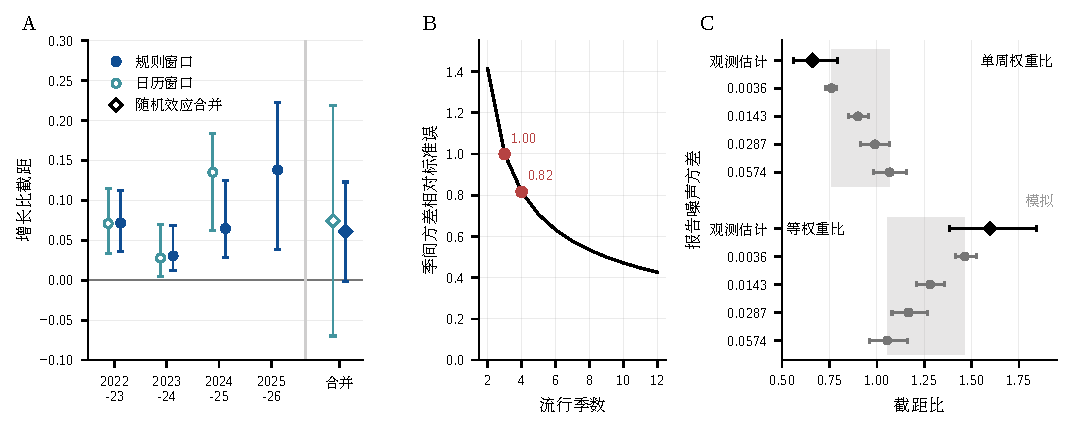
\includegraphics[width=0.86\linewidth]{figures/fig_07_seasons_pathogens_design.pdf}
  \caption{季间不确定性与分母权重比。（A）加权增长比的分季截距及双向自助 95\% 百分位区间，实心为规则窗口四季，空心为日历窗口三季；菱形为 DerSimonian--Laird 随机效应合并截距及 $t$ 分布 95\% 区间。（B）季间方差相对标准误的下界 $\sqrt{2/(S-1)}$ 随流行季数的变化，标出 $S=3$ 与 $S=4$。（C）规则窗口中单周分母比值 $q_1$ 与等权三周分母比值 $q_2$ 的估计（双向自助 95\% 百分位区间）与纯报告噪声零模型的比较。灰点为各报告噪声水平下比值的均值，误差线为其 2.5\%--97.5\% 分位范围（每个水平 300 条模拟路径，每条路径重新选择规则窗口），灰带为各水平均值的范围。}
  \label{fig:seasons}
\end{figure}

\FloatBarrier
\clearpage
\section{补充表格}
\label{app:tables}

\setcounter{table}{0}
\renewcommand{\thetable}{S\arabic{table}}

表~\ref{tab:s1}--\ref{tab:s6} 给出图~\ref{fig:floor}--\ref{fig:design} 与图~\ref{fig:seasons} 所依据的实证估计值，表~\ref{tab:s7} 汇总理论闭式量及其适用条件，表~\ref{tab:s8} 与表~\ref{tab:s9} 给出潜在环境方差反演在各设定下的结果与假设检验（图~\ref{fig:inversion}）。

\begin{table}[htbp]
\centering
\footnotesize
\setlength{\tabcolsep}{3pt}
\caption{各设定下相对损失的截距 $a$、斜率 $b$ 与表观平衡规模 $b/a$，附双向自助法 95\% 置信区间。}
\label{tab:s1}
\begin{tabular}{lrrcrccc r}
\toprule
设定 & $N$ & 周数 & 规模变量 & $\bar{x}$ & $a$ & $b$ & \begin{tabular}[t]{@{}c@{}}表观平衡\\规模 $b/a$\end{tabular} & \begin{tabular}[t]{@{}c@{}}标准差比\\（双向/州）\end{tabular} \\
\midrule
$R_A$，规则窗口（$S=4$） & 1748 & 42 & $C_t$ & 1.206 & \begin{tabular}[t]{@{}c@{}}0.0150\\ \relax[0.0100, 0.0205]\end{tabular} & \begin{tabular}[t]{@{}c@{}}0.560\\ \relax[0.375, 0.761]\end{tabular} & \begin{tabular}[t]{@{}c@{}}37.4\\ \relax[19.7, 69.7]\end{tabular} & 1.96 \\
$G$，规则窗口（$S=4$） & 1756 & 42 & $D_t$ & 1.724 & \begin{tabular}[t]{@{}c@{}}0.0840\\ \relax[0.0515, 0.1199]\end{tabular} & \begin{tabular}[t]{@{}c@{}}1.971\\ \relax[1.024, 3.005]\end{tabular} & \begin{tabular}[t]{@{}c@{}}23.5\\ \relax[8.8, 54.7]\end{tabular} & 2.19 \\
$R_A$，日历窗口（$S=3$） & 1263 & 29 & $C_t$ & 1.190 & \begin{tabular}[t]{@{}c@{}}0.0202\\ \relax[0.0104, 0.0307]\end{tabular} & \begin{tabular}[t]{@{}c@{}}0.516\\ \relax[0.284, 0.822]\end{tabular} & \begin{tabular}[t]{@{}c@{}}25.6\\ \relax[10.1, 73.9]\end{tabular} & 3.49 \\
$G$，日历窗口（$S=3$） & 1267 & 29 & $D_t$ & 1.671 & \begin{tabular}[t]{@{}c@{}}0.0991\\ \relax[0.0608, 0.1356]\end{tabular} & \begin{tabular}[t]{@{}c@{}}2.243\\ \relax[1.168, 3.550]\end{tabular} & \begin{tabular}[t]{@{}c@{}}22.6\\ \relax[9.4, 48.9]\end{tabular} & 2.52 \\
\bottomrule
\end{tabular}
\par\smallskip
\begin{minipage}{0.95\linewidth}\scriptsize 以迭代 FGLS 将 $L=((x-\bar{x})/\bar{x})^2$ 拟合为 $a+b/M$，$M$ 为规模变量且 $M\ge5$；$\bar{x}$ 为该设定合并窗口的均值（中心化层级：规格合并窗口）。区间为州$\times$周双向鸽笼自助法 95\% 百分位区间，$B=2000$，种子 20261029；各规格共享同一组州次数，周次数在季内按窗口抽取并由同一窗口的 $R_A$ 与 $G$ 共用，每次重抽重新估计中心化均值。标准差比为双向重抽与仅按州重抽（同一州次数）下 $a$ 的自助标准差之比。均为 51 个辖区。\end{minipage}
\end{table}

\begin{table}[htbp]
\centering
\footnotesize
\setlength{\tabcolsep}{3pt}
\caption{截距分解与自由幂律指数 $\gamma$，附双向自助法 95\% 置信区间。}
\label{tab:s2}
\begin{tabular}{lccccccc}
\toprule
设定 & $a$ 总量 & \begin{tabular}[t]{@{}c@{}}去除周效应\\后的 $a$\end{tabular} & \begin{tabular}[t]{@{}c@{}}去除周效应与\\州-季效应后的 $a$\end{tabular} & 周占比 & $\gamma$ & \begin{tabular}[t]{@{}c@{}}非收敛抽样\\占比（\%）\end{tabular} & \begin{tabular}[t]{@{}c@{}}仿射局部\\斜率均值\end{tabular} \\
\midrule
$R_A$，规则窗口（$S=4$） & \begin{tabular}[t]{@{}c@{}}0.0150\\ \relax[0.0100, 0.0205]\end{tabular} & \begin{tabular}[t]{@{}c@{}}0.0088\\ \relax[0.0066, 0.0122]\end{tabular} & \begin{tabular}[t]{@{}c@{}}0.0083\\ \relax[0.0066, 0.0137]\end{tabular} & \begin{tabular}[t]{@{}c@{}}0.41\\ \relax[0.12, 0.57]\end{tabular} & \begin{tabular}[t]{@{}c@{}}0.38\\ \relax[0.29, 0.51]\end{tabular} & 1.3 & $-$0.44 \\
$G$，规则窗口（$S=4$） & \begin{tabular}[t]{@{}c@{}}0.0840\\ \relax[0.0515, 0.1199]\end{tabular} & \begin{tabular}[t]{@{}c@{}}0.0415\\ \relax[0.0304, 0.0569]\end{tabular} & \begin{tabular}[t]{@{}c@{}}0.0394\\ \relax[0.0305, 0.0602]\end{tabular} & \begin{tabular}[t]{@{}c@{}}0.51\\ \relax[0.21, 0.65]\end{tabular} & \begin{tabular}[t]{@{}c@{}}0.35\\ \relax[0.21, 0.48]\end{tabular} & 0.3 & $-$0.38 \\
$R_A$，日历窗口（$S=3$） & \begin{tabular}[t]{@{}c@{}}0.0202\\ \relax[0.0104, 0.0307]\end{tabular} & \begin{tabular}[t]{@{}c@{}}0.0091\\ \relax[0.0068, 0.0126]\end{tabular} & \begin{tabular}[t]{@{}c@{}}0.0078\\ \relax[0.0056, 0.0145]\end{tabular} & \begin{tabular}[t]{@{}c@{}}0.55\\ \relax[0.11, 0.71]\end{tabular} & \begin{tabular}[t]{@{}c@{}}0.27\\（不报告）\end{tabular} & 14.4 & $-$0.33 \\
$G$，日历窗口（$S=3$） & \begin{tabular}[t]{@{}c@{}}0.0991\\ \relax[0.0608, 0.1356]\end{tabular} & \begin{tabular}[t]{@{}c@{}}0.0473\\ \relax[0.0353, 0.0652]\end{tabular} & \begin{tabular}[t]{@{}c@{}}0.0450\\ \relax[0.0326, 0.0901]\end{tabular} & \begin{tabular}[t]{@{}c@{}}0.52\\ \relax[0.24, 0.65]\end{tabular} & \begin{tabular}[t]{@{}c@{}}0.27\\（不报告）\end{tabular} & 13.8 & $-$0.33 \\
\bottomrule
\end{tabular}
\par\smallskip
\begin{minipage}{0.95\linewidth}\scriptsize 中心化层级：$a$ 总量按规格合并窗口均值；去除周效应时按同周辖区均值中心化，并乘 $n_w/(n_w-1)$ 校正自由度；州-季效应以周与州-季加性预测值（交替投影）中心化。周占比 $=1-a_{\text{去周}}/a_{\text{总量}}$，区间取自与分解相同的自助重抽；去除周效应给出统计上的方差划分，不作因果解释。$\gamma$ 为 $E(L)=cM^{-\gamma}$ 的全局拟合。非收敛抽样指 $\gamma>2$ 或 $\gamma<0$ 的自助重复；规则窗口中这类抽样不足 2\%，却使自助标准差膨胀十余倍。因此基于标准差的 Wald 检验与百分位区间对 $\gamma=1$ 的结论不一致，本表不报告检验 $p$ 值，百分位区间仅作描述。日历窗口的 $\gamma$ 自助分布严重重尾，区间不报告，亦不作推断依据。仿射局部斜率均值为 $-1/(1+M/(b/a))$ 在观测样本上的平均，仅为几何描述，与 $\gamma$ 没有相等关系。区间计算同表~\ref{tab:s1}。\end{minipage}
\end{table}

\begin{table}[htbp]
\centering
\footnotesize
\caption{医院报告完整度对截距贡献的等效性检验（TOST），附配对自助法 90\% 置信区间。}
\label{tab:s3}
\begin{tabular}{lcccccc c}
\toprule
设定 & $10^3\Delta a$ [90\% CI] & $10^3\delta_{0.10}$ & 等效 & $10^3\delta_{0.05}$ & 等效 & \begin{tabular}[t]{@{}c@{}}等效季数\\（$\tau_0=0.10$）\end{tabular} & \begin{tabular}[t]{@{}c@{}}等效季数\\（$\tau_0=0.05$）\end{tabular} \\
\midrule
$R_A$，规则窗口（$S=4$） & 0.29 [$-$0.24, 0.83] & 5.45 & 是 & 1.35 & 是 & 4/4 & 2/4 \\
$G$，规则窗口（$S=4$） & 0.37 [$-$2.76, 2.95] & 20.09 & 是 & 4.95 & 是 & 4/4 & 2/4 \\
$R_A$，日历窗口（$S=3$） & 0.09 [$-$0.48, 0.67] & 4.82 & 是 & 1.18 & 是 & 3/3 & 2/3 \\
$G$，日历窗口（$S=3$） & $-$0.38 [$-$3.68, 2.31] & 15.96 & 是 & 3.89 & 是 & 3/3 & 2/3 \\
\bottomrule
\end{tabular}
\par\smallskip
\begin{minipage}{0.95\linewidth}\scriptsize $\Delta a=a_{\text{原始}}-a_{\text{覆盖调整}}$，两者在同一覆盖有效子样本、同一规模变量上拟合，各按自身均值中心化。等效界 $\delta_{\tau_0}$ 为独立有界均匀乘性报告冲击（相对标准差 $\tau_0$，固定观测路径与规模，$R=2000$）下截距的平均增量，Monte Carlo 标准误不超过 0.205$\times10^{-3}$；该等效界依赖所设报告模型，用作敏感性校准。90\% 区间完全落在 $(-\delta,\delta)$ 内判为等效。区间为配对双向自助 90\% 百分位区间（同一重抽同时拟合原始与覆盖调整统计量），其余设定同表~\ref{tab:s1}。\end{minipage}
\end{table}

\begin{table}[htbp]
\centering
\footnotesize
\setlength{\tabcolsep}{3pt}
\caption{自愿报告期与同历月（5--10 月）的对照：$\log G$ 的四分位距及年份间比值。}
\label{tab:s4}
\begin{tabular}{llrrrccc}
\toprule
年份 & 报告制度 & $N$ & 周数 & $D_t$ 中位数 & $D_t$ 四分位 & $\log G$ 四分位距 [95\% CI] & $D$ 匹配四分位距 \\
\midrule
2023 & 强制 & 773 & 26 & 15.6 & 9.2--29.4 & 0.48 [0.40, 0.61] & 0.47 \\
2024 & 自愿 & 420 & 26 & 16.6 & 9.2--34.9 & 0.76 [0.48, 1.05] & 0.79 \\
2025 & 强制 & 841 & 26 & 16.2 & 9.6--29.6 & 0.48 [0.36, 0.58] & 0.50 \\
\midrule
比值 & 角色 & \multicolumn{2}{c}{95\% CI} & \multicolumn{2}{c}{90\% CI（次要）} & 单侧 $p$（次要） & $D$ 匹配比值 \\
\midrule
2024/2023 & 自愿/强制 & \multicolumn{2}{c}{1.58 [0.95, 2.23]} & \multicolumn{2}{c}{[1.01, 2.10]} & 0.046 & 1.68 \\
2024/2025 & 自愿/强制 & \multicolumn{2}{c}{1.57 [0.95, 2.39]} & \multicolumn{2}{c}{[1.03, 2.21]} & 0.041 & 1.58 \\
2025/2023 & 安慰剂 & \multicolumn{2}{c}{1.01 [0.72, 1.25]} & \multicolumn{2}{c}{[0.76, 1.21]} & 0.587 & 1.07 \\
\bottomrule
\end{tabular}
\par\smallskip
\begin{minipage}{0.95\linewidth}\scriptsize $\log G=\log\{(C_{t+1}+0.5)/(D_t+0.5)\}$，各年 5--10 月、$D_t\ge5$。区间由州次数跨年共享、周在年内独立抽样的双向自助法得到，$B=2000$，种子 20261941。主要比较为年份间四分位距比值的 95\% 区间；90\% 区间与单侧 $p$（自助分布落在比值 $\le1$ 一侧的比例）只作次要参考，未达 95\% 水平的结果不解释为确定差异。$D$ 匹配四分位距按 2023 与 2025 年合并的$\log D_t$ 十分位权重重新加权。2025/2023 为两个强制报告年份的安慰剂比较。\end{minipage}
\end{table}

\begin{table}[htbp]
\centering
\footnotesize
\setlength{\tabcolsep}{3pt}
\caption{分季截距（附双向自助法 95\% 置信区间）与季间异质性，四个设定分别报告。}
\label{tab:s5}
\begin{tabular}{lcccc}
\toprule
流行季 & \begin{tabular}[t]{@{}c@{}}$R_A$\\规则窗口（$S=4$）\end{tabular} & \begin{tabular}[t]{@{}c@{}}$G$\\规则窗口（$S=4$）\end{tabular} & \begin{tabular}[t]{@{}c@{}}$R_A$\\日历窗口（$S=3$）\end{tabular} & \begin{tabular}[t]{@{}c@{}}$G$\\日历窗口（$S=3$）\end{tabular} \\
\midrule
2022-23 & 0.0137 [0.0065, 0.0210] & 0.0718 [0.0358, 0.1126] & 0.0138 [0.0061, 0.0208] & 0.0711 [0.0335, 0.1150] \\
2023-24 & 0.0062 [0.0025, 0.0140] & 0.0305 [0.0126, 0.0686] & 0.0060 [0.0009, 0.0172] & 0.0277 [0.0049, 0.0694] \\
2024-25 & 0.0127 [0.0058, 0.0239] & 0.0647 [0.0290, 0.1244] & 0.0274 [0.0106, 0.0418] & 0.1352 [0.0626, 0.1838] \\
2025-26 & 0.0225 [0.0077, 0.0337] & 0.1383 [0.0386, 0.2230] & -- & -- \\
\midrule
$a_{\mathrm{RE}}$ [95\% CI] & 0.0123 [0.0021, 0.0225] & 0.0610 [$-$0.0010, 0.1231] & 0.0100 [$-$0.0037, 0.0236] & 0.0745 [$-$0.0697, 0.2186] \\
$Q$ ($p$) & 6.43 (0.092) & 5.81 (0.121) & 2.23 (0.328) & 9.77 (0.008) \\
$10^3\tau^2$ [Q-profile] & 0.021 [0.000, 0.601] & 0.704 [0.000, 26.738] & 0.004 [0.000, 4.210] & 2.647 [0.184, 114.920] \\
$I^2$ & 0.53 & 0.48 & 0.10 & 0.80 \\
\bottomrule
\end{tabular}
\par\smallskip
\begin{minipage}{0.95\linewidth}\scriptsize 中心化层级：分季截距按季内均值中心化。$a_{\mathrm{RE}}$ 为 DerSimonian--Laird 随机效应合并，区间用 $t_{S-1}$ 分位数；$\tau^2$ 区间为 Q-profile 95\% 区间\citep{viechtbauer2007confidence}。各季标准误取自同一双向自助输出。规则窗口 $S=4$，日历窗口 $S=3$（2025-26 季无日历窗口）。区间计算同表~\ref{tab:s1}。\end{minipage}
\end{table}

\begin{table}[htbp]
\centering
\footnotesize
\setlength{\tabcolsep}{3pt}
\caption{流感规则窗口（$S=4$）的权重比 $q_1$、$q_2$ 与纯报告噪声零模型的比较。}
\label{tab:s6}
\begin{tabular}{rrrcccc}
\toprule
$\mathrm{CV}^2$ & $R$ & 有效窗口 & $q_1$ 均值（MCSE） & $q_1$ 95\% 范围 & $q_2$ 均值（MCSE） & $q_2$ 95\% 范围 \\
\midrule
0.0036 & 300 & 262 & 0.760 (0.001) & [0.729, 0.786] & 1.464 (0.002) & [1.417, 1.525] \\
0.0143 & 300 & 231 & 0.900 (0.002) & [0.853, 0.955] & 1.282 (0.003) & [1.211, 1.356] \\
0.0287 & 300 & 238 & 0.990 (0.002) & [0.913, 1.065] & 1.167 (0.003) & [1.080, 1.267] \\
0.0574 & 300 & 208 & 1.067 (0.003) & [0.981, 1.158] & 1.055 (0.003) & [0.959, 1.161] \\
\midrule
\multicolumn{3}{l}{零模型范围（各格均值的极差）} & \multicolumn{2}{c}{0.760--1.067} & \multicolumn{2}{c}{1.055--1.464} \\
\multicolumn{3}{l}{敏感性：各季窗口均 $\ge4$ 周} & \multicolumn{2}{c}{0.762--1.077} & \multicolumn{2}{c}{1.051--1.462} \\
\multicolumn{3}{l}{观测（流感，$N=1756$）} & \multicolumn{2}{c}{0.660 [0.562, 0.792]} & \multicolumn{2}{c}{1.597 [1.384, 1.845]} \\
\multicolumn{3}{l}{观测落在零模型范围外的 $p$} & \multicolumn{2}{c}{0.120} & \multicolumn{2}{c}{0.217} \\
\bottomrule
\end{tabular}
\par\smallskip
\begin{minipage}{0.95\linewidth}\scriptsize $q_1=a_{\text{单周}}/a_{\text{原权重}}$，$q_2=a_{\text{等权}}/a_{\text{原权重}}$；各权重各自取 $D\ge5$ 且四周覆盖率为正的行。零模型条件于平滑的全国季节曲线与各州份额，只加入对数正态报告率（方差 $\mathrm{CV}^2$）与泊松计数噪声。每条模拟路径都按观测数据的规则重新选择窗口。任一季无法形成窗口的路径记为无效，不参与汇总；无效路径主要来自 2025-26 季起点处增长已低于 1 的情形。95\% 范围为模拟分布的 2.5\% 与 97.5\% 分位数，其分位点 CDF 尺度的 Monte Carlo 误差约 $\sqrt{0.025\cdot0.975/R_{\text{有效}}}\approx0.01$。该零模型不含传播增长、代际间隔与入院延迟。$p$ 为观测自助分布（$B=2000$，与 $G$ 规则窗口同一重抽流）落在零模型范围一侧比例的两倍，未做多重校正。\end{minipage}
\end{table}

\begin{table}[htbp]
\centering
\footnotesize
\setlength{\tabcolsep}{3pt}
\caption{理论闭式量、适用条件及基线数值。}
\label{tab:s7}
\begin{tabular}{p{0.2\linewidth}p{0.33\linewidth}p{0.27\linewidth}r}
\toprule
数量 & 闭式 & 条件 & 数值 \\
\midrule
$A$ & $\bar R+\rho(\bar R^2+v_R)/k$ & 固定 $\rho,k$ 与 $R$ 分布 & 2.123 \\
平衡规模 $m_\times$ & $A/v_R$ & $v_R>0$；经 $n$ 改变 $m=\rho n$ & 53.08 \\
规模倍增的相对降幅 & $1/[2(1+m/m_\times)]$ & 同上，$m=m_\times$ & 0.25 \\
报告概率倍增的相对降幅 & $\bar R/[2\rho n V(n,\rho)]$ & 固定 $n=m_\times/\rho=212.3$，$\rho\le1/2$ & 0.1354 \\
固定 $n$ 的可达下限 & $v_R+\bar R/n+(\bar R^2+v_R)/(kn)$ & $\rho\to1$，同上 $n$ & 0.0638 \\
$n$ 与 $\rho$ 的边际比 & $A/\bar R$ & 对数边际之比 & 1.846 \\
$v_H$ & $\tau^2(\bar R^2+v_R)$ & $\tau=0.15$ & 0.0307 \\
$m_{\times,H}$ & $A_H/(v_R+v_H)$ & $A_H=\bar R+\rho(1+\tau^2)(\bar R^2+v_R)/k$ & 30.36 \\
$m^*$ & $\sqrt{c_0A/(c_1v_R)}$ & 固定 $\rho$；$c_0/c_1=10$ & 23.04 \\
$m^*$ & $\sqrt{c_0A/(c_1v_R)}$ & 固定 $\rho$；$c_0/c_1=100$ & 72.86 \\
$\rho^*$ & $\sqrt{c_0Q/(c_\rho H)}$，截取到 $(0,1]$ & 固定 $n$；$c_0=100$，$c_\rho=c_1n$ & 0.2091 \\
$T^\dagger$ & $g_T=-T^2e^\prime(T)=1$ 的根 & $\phi=0.8$；一阶必要条件 & 4.484 \\
$B^\dagger$（$c_1$ 单位） & $T^\dagger(c_0+c_1m^*)$ & $c_0/c_1=100$；不含全局唯一性 & 775.0 \\
环境项（$\times10^{-3}$） & $v_RS(\phi,T)/T^2$ & $T=10$，$\phi=0.5$ & 10.40 \\
报告项（$\times10^{-3}$） & $\tau^2[\bar R^2S(\psi,T)+v_RS(\phi\psi,T)]/T^2$ & $\tau=0.15$，$\psi=0.5$ & 7.88 \\
抽样项（$\times10^{-3}$） & $A_H/(Tm)$ & $m=50$ & 4.29 \\
三项合计（$\times10^{-3}$） & 三项之和 & 同上 & 22.57 \\
Fisher 常数 & $\xi(\xi\psi_1(\xi)-1)$ & $\xi=\bar R^2/v_R=33.06$ & 0.505 \\
$v_R$ 相对标准误下界 & $[T\cdot\text{常数}]^{-1/2}$ & $T=10$ & 0.445 \\
季间方差 $v_S$ 相对标准误 & $\sqrt{2/(S-1)}$ & $S=3$，均值需估计 & 1.000 \\
季间方差 $v_S$ 相对标准误 & $\sqrt{2/(S-1)}$ & $S=4$，均值需估计 & 0.816 \\
报告冲击方差系数 & $1+\sum_jq_j^2$ & 平坦路径，$q=(0.65,0.25,0.10)$ & 1.4950 \\
相邻协方差系数 & $-q_1+\sum_kq_{1+k}q_k$ & 同上 & $-$0.4625 \\
均值偏差系数 & $\sum_jq_j^2$ & 同上 & 0.4950 \\
$\kappa(1)$ & $\alpha\beta$ & $g=1$，$\alpha=(3.6/1.6)^2$ & 0.5143 \\
\bottomrule
\end{tabular}
\par\smallskip
\begin{minipage}{0.95\linewidth}\scriptsize 基线 $\bar R=1.15$，$v_R=0.04$，$k=0.35$，$\rho=0.25$。平衡规模 $m_\times$ 为理论量，与经验拟合的表观平衡规模 $b/a$ 之间需要明确校准映射，不恒等。$e(T)=S(\phi,T)/T^2$，$S(\phi,T)=\sum_{|h|<T}(T-|h|)\phi^{|h|}$；$\psi$ 为相对报告扰动项 $\varepsilon_t=p_t/\rho-1$ 的一阶自相关系数。报告冲击三项系数乘 $\tau^2$ 给出二阶近似，需分母远离零与一致可积条件；非平坦增长路径下 $q$ 需重算。全部数值由闭式计算并经数值核对。\end{minipage}
\end{table}

\begin{table}[htbp]
\centering
\footnotesize
\setlength{\tabcolsep}{4pt}
\caption{两步反演在各模拟设定下给出的隐含环境方差 $v_R^{\mathrm{impl}}$，以及各估计值的 95\% 置信区间。}
\label{tab:s8}
\begin{tabular}{lllrrll}
\toprule
设定 & 由 $R_A$ 得到的 $v_R^{\mathrm{impl}}$ & 由 $G$ 得到的 $v_R^{\mathrm{impl}}$ & $\kappa_{R_A}$ & $\kappa_G$ & 比值 $R_A/G$ & 一致 \\
\midrule
数据匹配设计（M0） & 0.040 [0.026, 0.056] & 0.043 [0.025, 0.064] & 0.516 & 2.729 & 0.93 [0.78, 1.18] & 是 \\
无全国冲击 & 0.039 [0.026, 0.055] & 0.042 [0.024, 0.062] & 0.523 & 2.775 & 0.94 [0.79, 1.18] & 是 \\
全国份额 0.65 & 0.040 [0.026, 0.056] & 0.043 [0.025, 0.065] & 0.510 & 2.670 & 0.92 [0.77, 1.16] & 是 \\
AR(1)，$\phi=0.5$ & 0.027 [0.017, 0.040] & 0.025 [0.013, 0.039] & 0.780 & 4.699 & 1.08 [0.88, 1.43] & 是 \\
真实代际间隔均值 2.2 天 & 0.013 [0.008, 0.019] & 0.014 [0.008, 0.021] & 1.287 & 6.991 & 0.94 [0.77, 1.20] & 是 \\
真实代际间隔均值 4.3 天 & 0.058 [0.038, 0.081] & 0.063 [0.037, 0.095] & 0.380 & 1.977 & 0.92 [0.77, 1.16] & 是 \\
延迟均值 3.5 天 & 0.038 [0.025, 0.053] & 0.041 [0.024, 0.061] & 0.535 & 2.790 & 0.93 [0.77, 1.16] & 是 \\
延迟均值 8 天 & 0.046 [0.030, 0.064] & 0.047 [0.027, 0.069] & 0.454 & 2.483 & 0.98 [0.82, 1.22] & 是 \\
$k=0.1$ & 0.040 [0.026, 0.055] & 0.042 [0.025, 0.062] & 0.517 & 2.740 & 0.94 [0.79, 1.18] & 是 \\
报告计数同步冲击 & 0.019 [0.006, 0.035] & 0.029 [0.012, 0.048] & 1.041 & 4.553 & 0.67 [0.39, 0.90] & 否 \\
通用独立面板设计 & 0.043 [0.029, 0.059] & 0.044 [0.027, 0.063] & 0.507 & 2.734 & 0.97 [0.83, 1.18] & -- \\
\bottomrule
\end{tabular}
\par\smallskip
\begin{minipage}{0.95\linewidth}\scriptsize 各设定只改变数据匹配设计中的一个要素（第~\ref{sec:meth-inversion}~节），分析者所用代际间隔的均值始终为 3.6 天。区间合并了两个实证截距的 2000 次联合双向自助抽样，以及校准线按其蒙特卡罗抽样分布的抽取。$\kappa=\E(\hat{a})/(v_R/\bar{R}^2)$，取最接近隐含方差的 $v_R$ 格点值。“一致”表示两个隐含方差之差的 95\% 区间包含零；通用独立面板设计（第~\ref{sec:meth-sim}~节）用于对照，不计入十种设定。\end{minipage}
\end{table}

\begin{table}[htbp]
\centering
\footnotesize
\setlength{\tabcolsep}{4pt}
\caption{滞后一阶自相关以及补充反演设定下的隐含环境方差与 $b/a$。}
\label{tab:s9}
\begin{tabular}{lllll}
\toprule
\multicolumn{5}{l}{\textit{A. 滞后一阶自相关}}\\
设定 & $R_A$ 的 $r_1$ & 数据分位 & $G$ 的 $r_1$ & 数据分位 \\
\midrule
数据（规则窗口） & $-$0.095 [$-$0.168, $-$0.019] & -- & 0.123 [0.039, 0.201] & -- \\
数据匹配设计（M0） & $-$0.074 [$-$0.151, 0.014] & 31.0 & 0.114 [0.025, 0.220] & 62.0 \\
AR(1)，$\phi=0.25$ & 0.007 [$-$0.098, 0.118] & 3.0 & 0.193 [0.097, 0.304] & 10.0 \\
AR(1)，$\phi=0.5$ & 0.072 [$-$0.039, 0.229] & 0.0 & 0.258 [0.146, 0.390] & 0.0 \\
真实代际间隔均值 2.2 天 & 0.099 [$-$0.002, 0.223] & 0.0 & 0.251 [0.156, 0.363] & 0.0 \\
真实代际间隔均值 2.9 天 & 0.006 [$-$0.083, 0.120] & 2.5 & 0.183 [0.091, 0.296] & 9.0 \\
真实代际间隔均值 4.3 天 & $-$0.134 [$-$0.206, $-$0.030] & 80.0 & 0.051 [$-$0.031, 0.161] & 92.0 \\
住院数方差均值比 1.5 & $-$0.170 [$-$0.233, $-$0.096] & 97.5 & $-$0.014 [$-$0.092, 0.076] & 100.0 \\
住院数方差均值比 2.0 & $-$0.183 [$-$0.247, $-$0.104] & 99.0 & $-$0.041 [$-$0.104, 0.035] & 100.0 \\
报告计数同步冲击 & $-$0.146 [$-$0.225, $-$0.076] & 86.0 & 0.041 [$-$0.033, 0.116] & 99.0 \\
\midrule
\multicolumn{5}{l}{\textit{B. 补充设定（$b/a$ 取 $v_R=0.04$ 处的汇总值）}}\\
设定 & 由 $R_A$ 得到的 $v_R^{\mathrm{impl}}$ & 由 $G$ 得到的 $v_R^{\mathrm{impl}}$ & $R_A$ 的 $b/a$ & $G$ 的 $b/a$ \\
\midrule
数据匹配设计（M0） & 0.040 [0.026, 0.056] & 0.043 [0.025, 0.064] & 28.0 & 16.2 \\
真实代际间隔均值 2.9 天 & 0.026 [0.017, 0.036] & 0.027 [0.016, 0.040] & 18.2 & 10.4 \\
住院数方差均值比 1.5 & 0.039 [0.026, 0.055] & 0.044 [0.026, 0.066] & 68.0 & 40.2 \\
住院数方差均值比 2.0 & 0.039 [0.026, 0.055] & 0.045 [0.027, 0.066] & 81.0 & 48.4 \\
AR(1)，$\phi=0.25$ & 0.033 [0.021, 0.047] & 0.033 [0.019, 0.049] & 23.4 & 12.6 \\
\bottomrule
\end{tabular}
\par\smallskip
\begin{minipage}{0.95\linewidth}\scriptsize $r_1$ 为州--季节块内相对偏差 $x/\bar{x}_{\text{块}}-1$ 的汇总滞后一阶自相关。数据行的区间来自按州整群的自助抽样（1000 次）；模拟行给出 $v_R=0.04$ 时各面板 $r_1$ 的均值及 2.5\%--97.5\% 分位范围（B 部分各设定每个 $v_R$ 取 200 个面板，其余设定取 100 个），“数据分位”为数据值在模拟分布中的百分位。分析者所用代际间隔均值始终为 3.6 天；2.9 天与 4.3 天对应 \citet{cowling2009estimation} 所估流感序列间隔的 95\% 区间端点。住院数方差均值比通过对每周住院数施加伽马--泊松混合实现。\end{minipage}
\end{table}

